\subsection{Comparison with the Baseline}
Table~\ref{tab:main} and Fig.~\ref{fig:core} report the macro-averages and paired statistics. \sys scores higher on every metric, and its largest and only significant advantage after correction is in \textbf{Relevancy}: \RelSys\% versus \RelBase\% (+\RelDiff{} percentage points (pp); 95\% CI [30.9, 53.2]; $p_{\mathrm{Holm}}=4.6\times10^{-5}$; rank-biserial $r=0.99$). \sys was more relevant on 25 of 30 products and less relevant on only one. This confirms statistically that the baseline's extra scene content is largely irrelevant to the purchase decision.

\textbf{Objectivity} (+4.72~pp, $p=0.023$) and \textbf{Relevant Novelty} (+13.84~pp, $p=0.015$) have confidence intervals that exclude zero and medium-to-large effect sizes ($r=0.67$ and $0.53$), but they do not survive Holm correction ($p_{\mathrm{Holm}}=0.069$ and $0.061$). We therefore report them as consistent trends. Relevant Novelty favored \sys on 20 products versus 7. \textbf{Avoidable Redundancy} (17.76\% vs.\ 20.55\%) and \textbf{Information Efficiency} (5.94 vs.\ 4.93 relevant novel claims per 100 words) favor \sys on average, but their differences are small relative to between-image variation ($p_{\mathrm{Holm}}=0.83$). \sys's higher rate of \emph{unavoidable} repetition (41.25\% vs.\ 19.35\%) is intended: it reflects anchor phrases that make new visual relations understandable and is not penalized.

\begin{figure}[t]
\centering
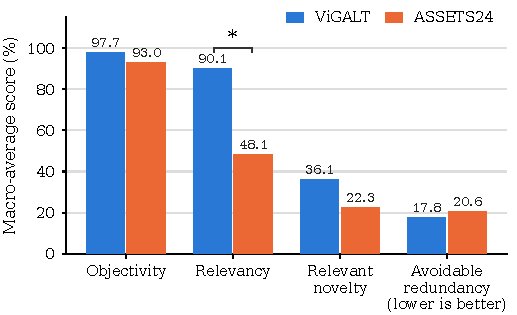
\includegraphics[width=\columnwidth]{figures/core_metrics_vigalt.pdf}
\caption{Macro-averaged claim-level scores for \sys and \base on the 30 paired products (Avoidable Redundancy: lower is better). $^{*}$Significant after Holm correction.}
\label{fig:core}
\end{figure}

\begin{table}[t]
\caption{Macro-averaged results ($n=30$ paired products). $\Delta$ = \sys $-$ \base, in pp (Efficiency: relevant novel claims per 100 words).}
\label{tab:main}
\centering
\footnotesize
\setlength{\tabcolsep}{2.4pt}
\begin{tabular}{@{}lrrcrr@{}}
\toprule
Metric & \sys & \base & $\Delta$ [95\% CI] & $p_{\mathrm{Holm}}$ & $r$ \\
\midrule
Relevancy $\uparrow$        & \textbf{\RelSys} & \RelBase & +\RelDiff{} [30.9, 53.2] & $<$0.001$^{*}$ & 0.99 \\
Objectivity $\uparrow$& \textbf{97.71} & 92.99 & +4.72 [1.2, 8.4]   & 0.069 & 0.67 \\
Rel.\ Novelty $\uparrow$    & \textbf{36.12} & 22.29 & +13.84 [3.1, 24.2] & 0.061 & 0.53 \\
Avoid.\ Red. $\downarrow$& \textbf{17.76} & 20.55 & $-$2.80 [$-$9.2, 3.3] & 0.828 & 0.14 \\
Efficiency $\uparrow$      & \textbf{5.94}  & 4.93  & +1.01 [$-$1.0, 3.0] & 0.828 & 0.18 \\
\bottomrule
\end{tabular}\\[2pt]
\parbox{\columnwidth}{\scriptsize $^{*}$Significant at $\alpha=0.05$ after Holm correction ($p_{\mathrm{Holm}}=4.6\times10^{-5}$). $r$: matched-pairs rank-biserial correlation. Bold: better value.}
\end{table}

Fig.~\ref{fig:cases} illustrates the relevancy gap: \base spends much of its description on the model's accessories and bottoms and on the nursery's decor, whereas \sys describes the T-shirt's cut and chest graphic and the bed frame itself.

\begin{figure}[t]
\centering
\scriptsize
\begin{minipage}[t]{0.25\columnwidth}\vspace{0pt}\centering
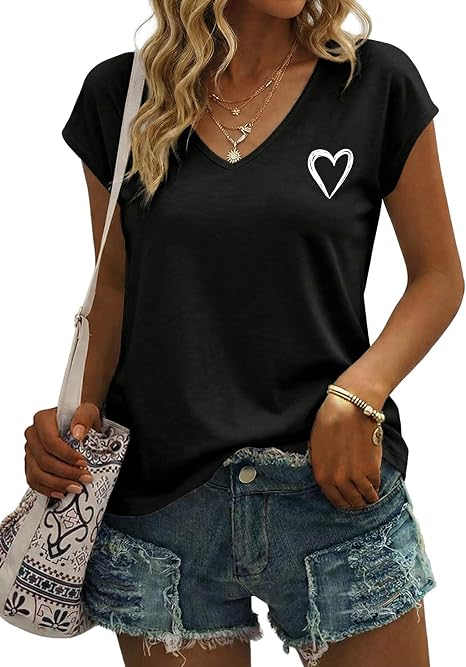
\includegraphics[width=\linewidth]{figures/case_clothing_02.jpg}\\(a) Clothing
\end{minipage}\hfill
\begin{minipage}[t]{0.72\columnwidth}\vspace{0pt}
\textbf{\base:} A woman wears a black V-neck T-shirt with a white heart outline, \textcolor{red}{layered necklaces}, and \textcolor{red}{bracelets}, paired with \textcolor{red}{distressed blue denim shorts}. A \textcolor{red}{patterned shoulder bag hangs at her side}.\\[2pt]
\textbf{\sys:} A T-shirt is shown worn on a person. It has a V-neckline, a straight body extending to the upper hips, and short sleeves ending above the elbows, with an irregular white outlined heart on the upper right chest.
\end{minipage}\\[5pt]
\begin{minipage}[t]{0.25\columnwidth}\vspace{0pt}\centering
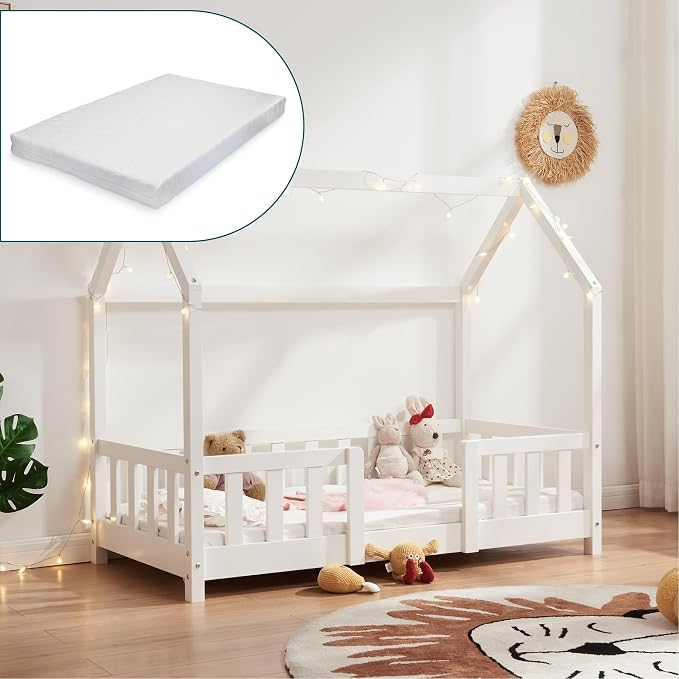
\includegraphics[width=\linewidth]{figures/case_furniture_24.jpg}\\(b) Furniture
\end{minipage}\hfill
\begin{minipage}[t]{0.72\columnwidth}\vspace{0pt}
\textbf{\base:} Bright nursery with a \textcolor{red}{white house-style crib, pink-and-white bedding}, plush toys, and string lights. \textcolor{red}{A plush lion hangs on the wall}, while a \textcolor{red}{crocheted toy lies on the wooden floor} beside an animal-patterned rug. A rounded inset in the upper left shows a white crib mattress. White walls and pale curtains complete the room.\\[2pt]
\textbf{\sys:} A white-painted bed frame has a peaked roof-shaped frame with four corner posts. Raised guard panels made of vertical slats run along the sides and foot end, with a solid back panel behind the low-set sleeping surface and an opening at the front. The sleeping surface contains a white mattress with a lightly quilted cover.
\end{minipage}
\caption{Qualitative comparison. \textcolor{red}{Red} marks purchase-irrelevant detail in \base; \sys text is unmarked.}
\label{fig:cases}
\end{figure}

